\chapter{Crecimiento de films de MgB$_2$ por evaporación}\label{C:evap}
\graphicspath{{figs/evap/}}

\chapterquote{La vida es como el Tetris, los errores se acumulan y los aciertos desaparecen}{Dicho popular}
%%%%%%%%%%%%%%%%%%%%%%%%%%%%%%%%%%%%%%%%%%%%%%%%%%%%%%%%%%%%%%%%%%%%%%%%
En este capítulo se muestran los resultados obtenidos al intentar fabricar films superconductores de MgB$_{2}$, mediante una técnica que consistió en evaporar films de boro sobre un sustrato, para luego recocer en una ampolla de cuarzo los mismos films junto con una pastilla bulk de MgB$_{2}$ obtenida comercialmente. Los sustratos elegidos fueron zafiro y silicio, dos materiales que poseen una baja conductividad eléctrica y elevada conductividad térmica a bajas temperaturas. El silicio presenta la ventaja adicional de que puede ser fácilmente micromaquinado por procedimientos estándar. Se muestran además mediciones del espesor de los films utilizando un perfilómetro mecánico y la caracterización de las propiedades magnéticas obtenidas a partir de mediciones en un magnetómetro SQUID. La técnica de crecimiento empleada en este capítulo posee la ventaja de ser muy sencilla de implementar pero posee las desventajas de ser un proceso poco repetible que involucra elevadas temperaturas para poder funcionar bien. El mayor problema con los procesos que requieren elevadas temperaturas es que los mismos son más susceptibles a contaminación. Por ejemplo, a altas temperaturas el oxígeno del zafiro puede reaccionar con el magnesio que se quiere depositar en el film de boro, lo que produce un ensanchamiento de la transición superconductora, empeorando el rendimiento del detector.

\section{Procedimiento}\label{S:evapproc}
La fabricación de las muestras por evaporación se realizó en dos etapas: en la primera etapa se evaporó B sobre diferentes sustratos y en la segunda se hizo un recocido de los films evaporados encapsulados junto a muestras bulk de MgB$_2$. Como sustratos se eligieron monocristales de silicio (111) y zafiro (0001). Se utilizaron estos sustratos porque, dentro de los disponibles en el laboratorio, presentan propiedades que interesan para la construcción del detector, básicamente una buena conductividad térmica y son aisladores\cite{Ekin2006}. El objetivo del recocido es colocar a los films de boro en un ambiente en el que estén en equilibrio con la presión de vapor de la muestra bulk de MgB$_2$\cite{Barrabas2011}. En una situación así se busca igualar los potenciales químicos de ambos materiales, lo que implica que los films de boro incorporarán magnesio hasta tener una composición idéntica a la de la muestra bulk. La evaporación de boro sobre el sustrato se hizo en un equipo como el que se esquematiza en la Fig.\,\ref{fig:eva}.
\begin{figure}[tbh!]
 \begin{center}
    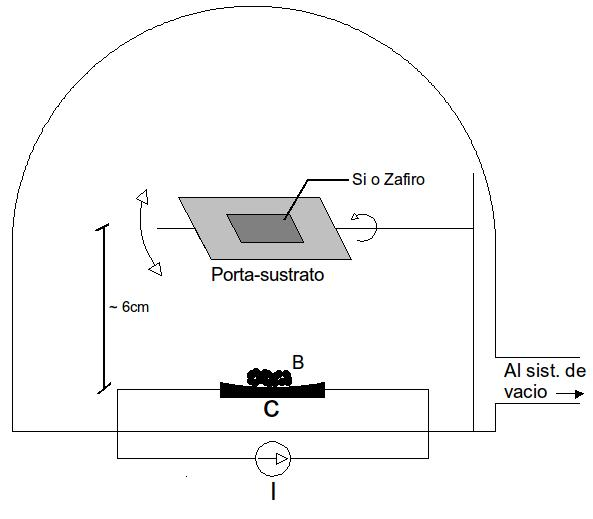
\includegraphics[width=0.6\columnwidth]{evaporadora1}
  \end{center}
  \caption[Esquema del arreglo utilizado para evaporar boro sobre diferentes sustratos.]{Esquema del arreglo utilizado para evaporar boro sobre diferentes sustratos. I es la fuente de corriente
que se utilizó para hacer pasar corriente sobre la naveta C, sobre la que depositó el boro. El interior de la campana se encontraba en condición de alto vacío ($P \sim 10^{-6}$\,Torr).}
\label{fig:eva}
\end{figure}
%\newpage
El boro se evaporó desde una naveta de grafito tallada especialmente (Fig.\,\ref{fig:nav}). Las navetas se angostaron de modo de aumentar la densidad de corriente en el centro de la misma, y se pusieron en serie con una fuente de corriente que podía entregar hasta 150\,Ampere. El sustrato se colocó en el porta-sustrato y se ubicó por sobre la naveta. El depósito de boro se hizo en condiciones de alto vacío ($p$ $\sim$ $10^{-6}$\,Torr).
\begin{figure}[tbh!]
 \begin{center}
    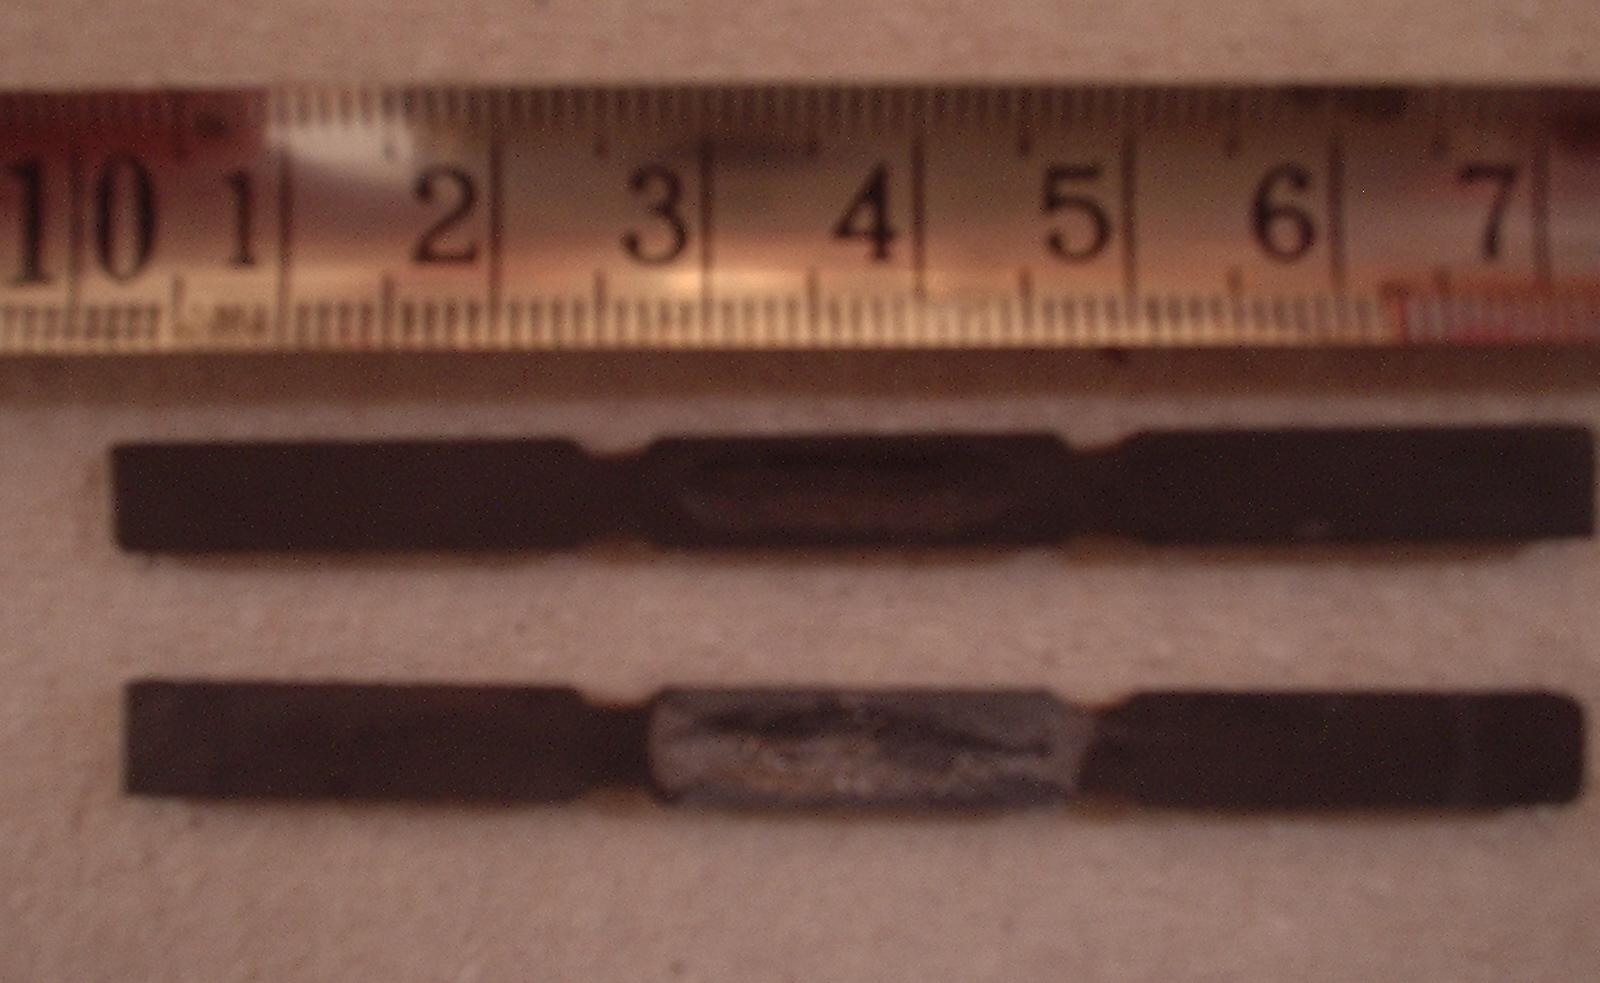
\includegraphics[width=0.5\columnwidth]{navetas}
  \end{center}
  \caption[Las navetas de grafito utilizadas para la evaporación.]{Las navetas de grafito utilizadas para la evaporación. Las mismas fueron talladas especialmente
de modo de incrementar la densidad de corriente en las regiones en las que se depositaba el boro. Puede apreciarse
la diferencia de cómo se veían las navetas antes de la evaporación (arriba) y después de la misma (abajo).}
  \label{fig:nav}
\end{figure}
\nomenclature{$p$}{Presión hidrostática.}
\newpage
Una vez crecidos los films, se colocaron en un tubo de cuarzo junto con una pastilla de MgB$_2$ envuelta en una lámina de tantalio, como se ve en la Fig.\ref{fig:tubos}. El tantalio evita la oxidación de los films, ya que absorbe el oxígeno que desgasa la pastilla de MgB$_2$ durante el recocido\cite{Barrabas2011}.
El tubo de cuarzo así sellado se colocó en un horno donde se realizó el recocido a diferentes temperaturas y por diferentes períodos de tiempo, alrededor de los 700 ºC y las 20 hs, respectivamente.
\begin{figure}[tbh!]
 \begin{center}
    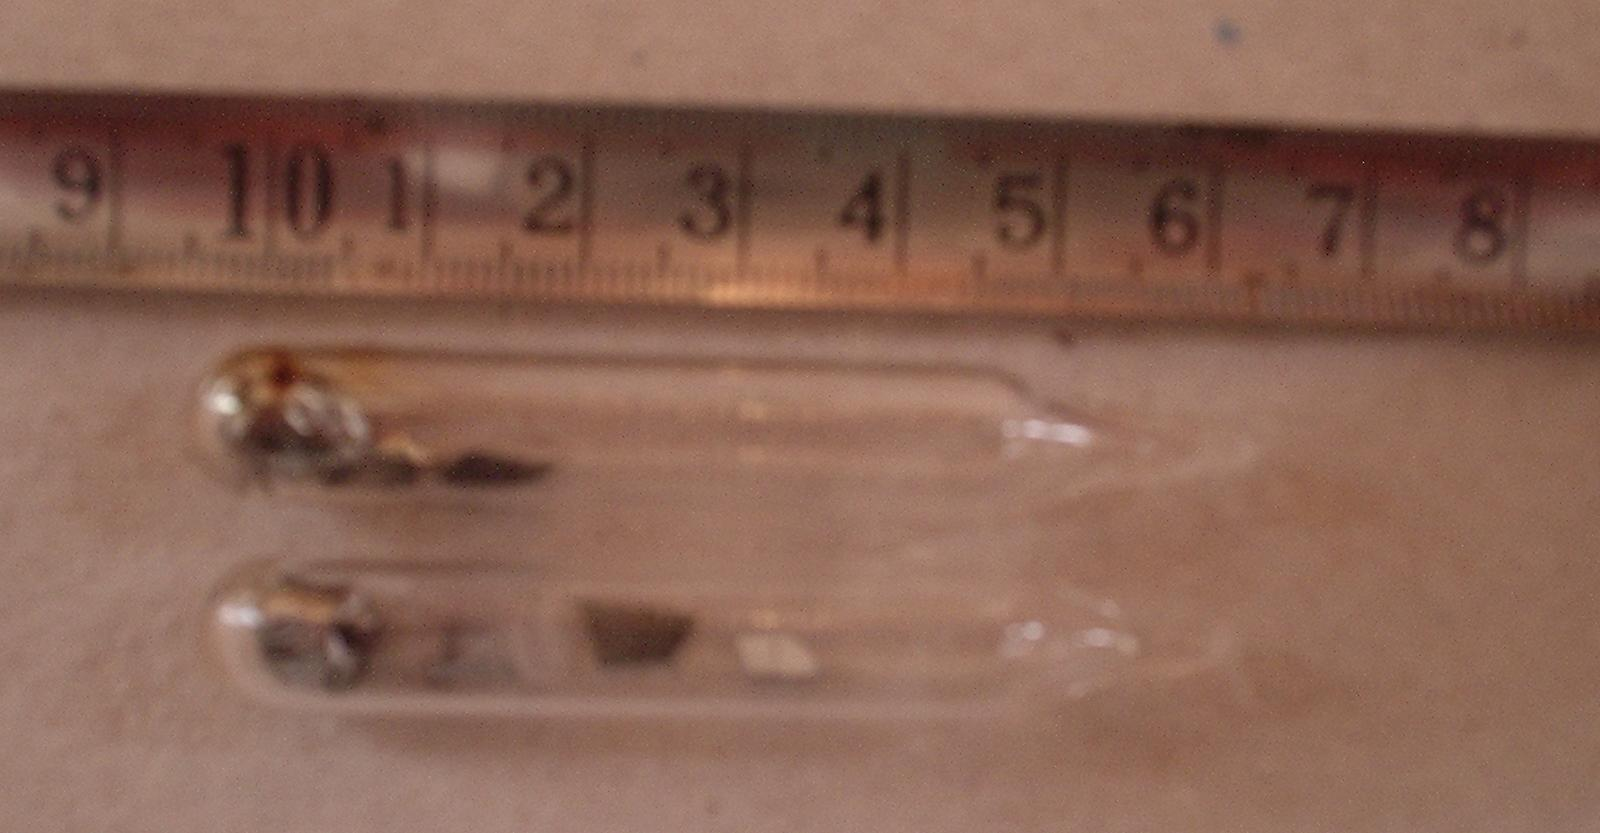
\includegraphics[width=0.5\columnwidth]{tubos}
  \end{center}
\caption[Tubos de cuarzo utilizados para recocer los films de boro con pastillas de MgB$_2$.]{Tubos de cuarzo utilizados para recocer los films de boro con pastillas de MgB$_2$. El MgB$_2$ fue envuelto 
en una lámina de tantalio para evitar la oxidación de los films.}
\label{fig:tubos}
\end{figure}

Los films obtenidos fueron caracterizados en un magnetómetro SQUID en donde se midió su magnetización en función de la temperatura durante un proceso \textit{Zero field cooling - Field cooling} (ZFC-FC). El SQUID es un dispositivo que consiste en un arreglo de junturas Josephson que permiten medir campos magnéticos con elevada precisión y bajos niveles de ruido, por lo que resulta un equipo muy útil para determinar la magnetización de films, que son materiales con masas pequeñas, y que por ende producen señales magnéticas también pequeñas. El proceso ZFC-FC consiste en llevar al superconductor a una temperatura $T\ < \ T_{c}$, a campo nulo, para luego aplicar un campo magnético $H \ < H_c$ (proceso \textit{Zero Field Cooling}). Como en el interior de un superconductor se tiene $B\ = \ 0$, el SQUID registra una señal diamagnética que proviene de la muestra, es decir que se tiene $M \, < \, 0$. El paso siguiente del proceso es calentar el sistema, con campo aplicado, hasta que se tiene $T \ > \ T_c$, lo que lleva al material al estado normal. Es esta circunstancia, el campo magnético penetra en el superconductor y el SQUID registra una señal nula, o sea, $M \ = \ 0$. El paso final del proceso consiste en enfriar nuevamente a $T \ < \ T_c$ con campo aplicado (proceso \textit{Field Cooling}). Sin embargo, como el campo ya penetró en el material, cuando se cumple $T \ < \ T_c$, la expulsión del campo magnético no es completa, lo que implica que se observa una irreversibilidad en el gráfico $M \ vs \ T$ cuando el superconductor es sometido a un proceso ZFC-FC.
\nomenclature{$H$}{Campo magnético aplicado.}

La medición de magnetización en un proceso de este estilo es una técnica estándar utilizada para la determinación del carácter superconductor de un film, así como un método muy preciso para determinar su $T_{c}$.

El ciclo ZFC-FC elegido para caracterizar las muestras consistió en llevar la muestra a 5\,K a campo nulo y aplicar un campo magnético. A continuación se incrementó lentamente la temperatura de la muestra hasta $T \ = 45$\,K, que es una temperatura mayor que la mayor $T_c$ esperable para el MgB$_2$. Luego se enfrió nuevamente la muestra hasta $T\ = 5$\,K con campo aplicado. En la Fig.\,\ref{fig:bulk} se muestra, a modo de ejemplo, la curva de magnetización de la pastilla de MgB$_2$ utilizada para generar los films.
\begin{figure}[tbh!]
 \begin{center}
    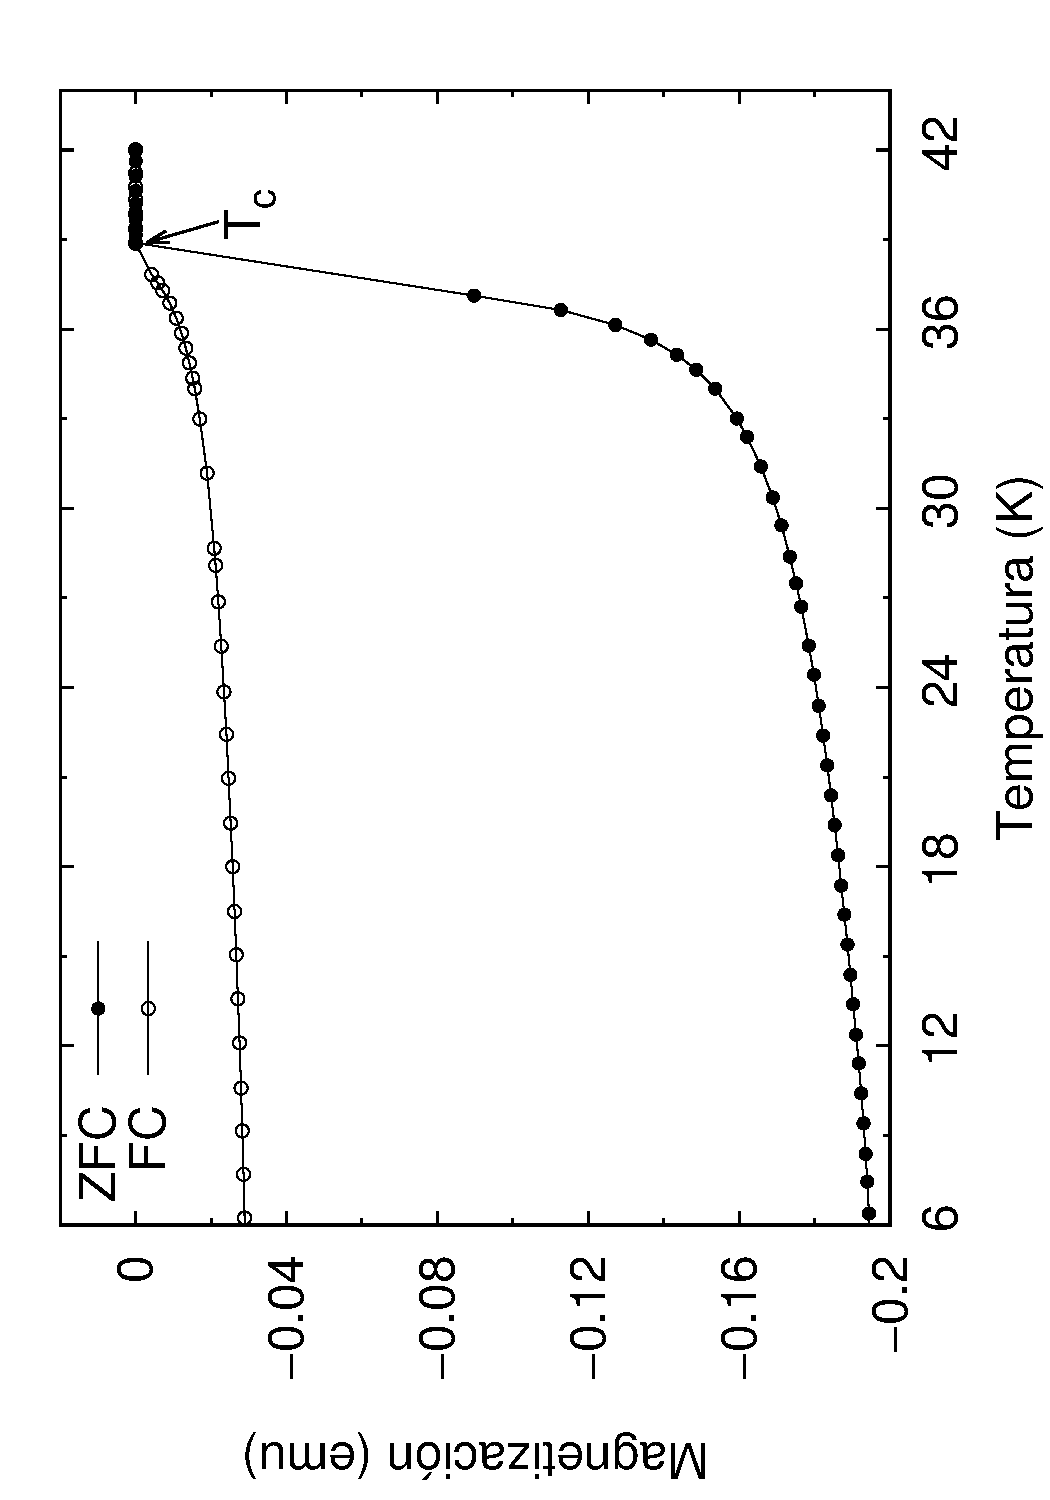
\includegraphics[width=0.5\columnwidth, angle=-90]{mgb2bulk}
  \end{center}
\caption{Curvas de magnetización en un proceso ZFC-FC de la pastilla de MgB$_2$ utilizada para generar los films.}
\label{fig:bulk}
\end{figure}
%\newpage
En este trabajo se realizaron tres evaporaciones con sus correspondientes recocidos: la primera con sustratos del silicio y las otras dos con sustratos de silicio y zafiro. Las muestras de la segunda evaporación se recocieron mezclando en el tubo de cuarzo muestras con sustratos de silicio y zafiro y las de la tercera recociendo por separado el zafiro y el silicio. Las muestras de la primera evaporación estaban muy contaminadas y no resultaron ser superconductoras.

\section{Caracterización de los films de MgB$_2$}\label{S:evapcarac}
Se presenta a continuación la caracterización realizada sobre las distintas muestras fabricadas. Tal como se comentó previamente, los films de la primera evaporación estaban demasiado contaminados y, debido a eso, no eran superconductores. En la tabla\,\ref{tab:muestras} se muestran resumidos los datos obtenidos de las distintas muestras. Sólo aparecen los datos de la segunda y la tercera evaporación.
\begin{table}[h!]
\centering
\begin{tabular}{|c|c|c|c|c|c|} \hline
  N$^{\circ}$ de Evap.& Muestras & Sustrato & $T_{rec}$(C) & $t_{rec}$(hs.) & Espesor (nm) \\ \hline
2 & BBSi 1 a 4&Si (111)&750&20&$(540 \, \pm \, 50)$ \\
2 & BBZ 1 a 3&Al$_2$O$_3$ (0001)&750&20&$(540 \, \pm \, 50)$  \\ \hline
3 & BBSi 5 a 9&Si (111)&700&20&$(80 \, \pm \, 10)$ \\
3 & BBZ 4 a 8&Al$_2$O$_3$ (0001)&700&20&$(80 \, \pm \, 10)$\\ \hline
\end{tabular}
\caption[Las muestras producidas por medio del método de evaporación y recocido.]{Las muestras producidas en esta etapa del trabajo. Se muestran los tiempos y temperaturas de los recocidos,
el sustrato en el que fueron crecidas las muestras y el espesor estimado de las mismas.}
\label{tab:muestras}
\end{table} 

A modo de ejemplo, se muestran en las Figs.\,\ref{fig:mgb2si} y \ref{fig:mgb2zaf} curvas representativas de magnetización en función de la temperatura para dos de las muestras fabricadas, una depositada sobre sustrato de silicio y otra sobre sustrato de zafiro. La curva de magnetización en función de la temperatura del film BBSi 3 aparece en la Fig.\,\ref{fig:mgb2si}.
\begin{figure}[h!]
 \begin{center}
    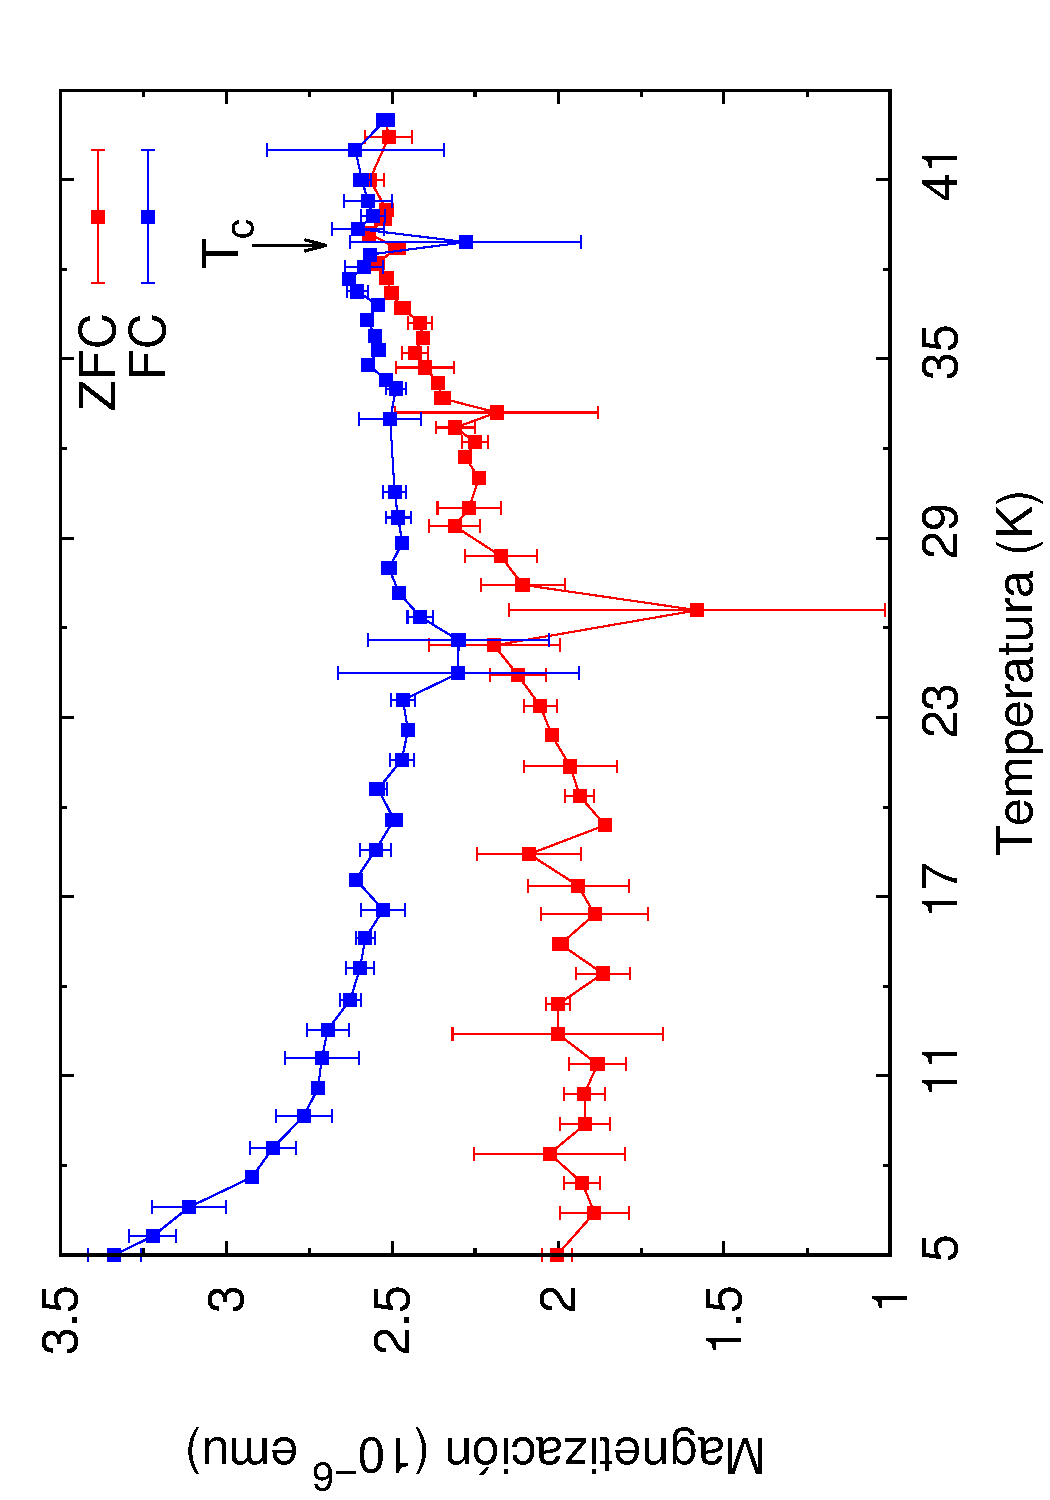
\includegraphics[width=0.5\columnwidth, angle=-90]{mgb2si}
  \end{center}
\caption[Magnetización en función de la temperatura para la muestra BBSi 3.]{Magnetización en función de la temperatura para la muestra BBSi 3. El sustrato es de Si. El hecho de que la señal sea positiva se debe al paramagnetismo del silicio. Sin embargo puede apreciarse una irreversibilidad que indica una transición superconductora cuya $T_c$ se encuentra entre 36\,K y 38\,K.}
\label{fig:mgb2si}
\end{figure}
\newpage
Puede verse que la curva de magnetización de la figura\,\ref{fig:mgb2si} es cualitativamente si\-mi\-lar a la obtenida al medir la pastilla de MgB$_2$ utilizada para hacer el recocido de los films (ver Fig.\,\ref{fig:bulk}). La irreversibilidad de la curva de magnetización sugiere que existe una transición superconductora a una $T_c$ algo menor que 38\,K. El hecho de que la señal sea positiva se debe al paramagnetismo del sustrato de Si\cite{Barrabas2011}.
\begin{figure}[h!]
 \begin{center}
    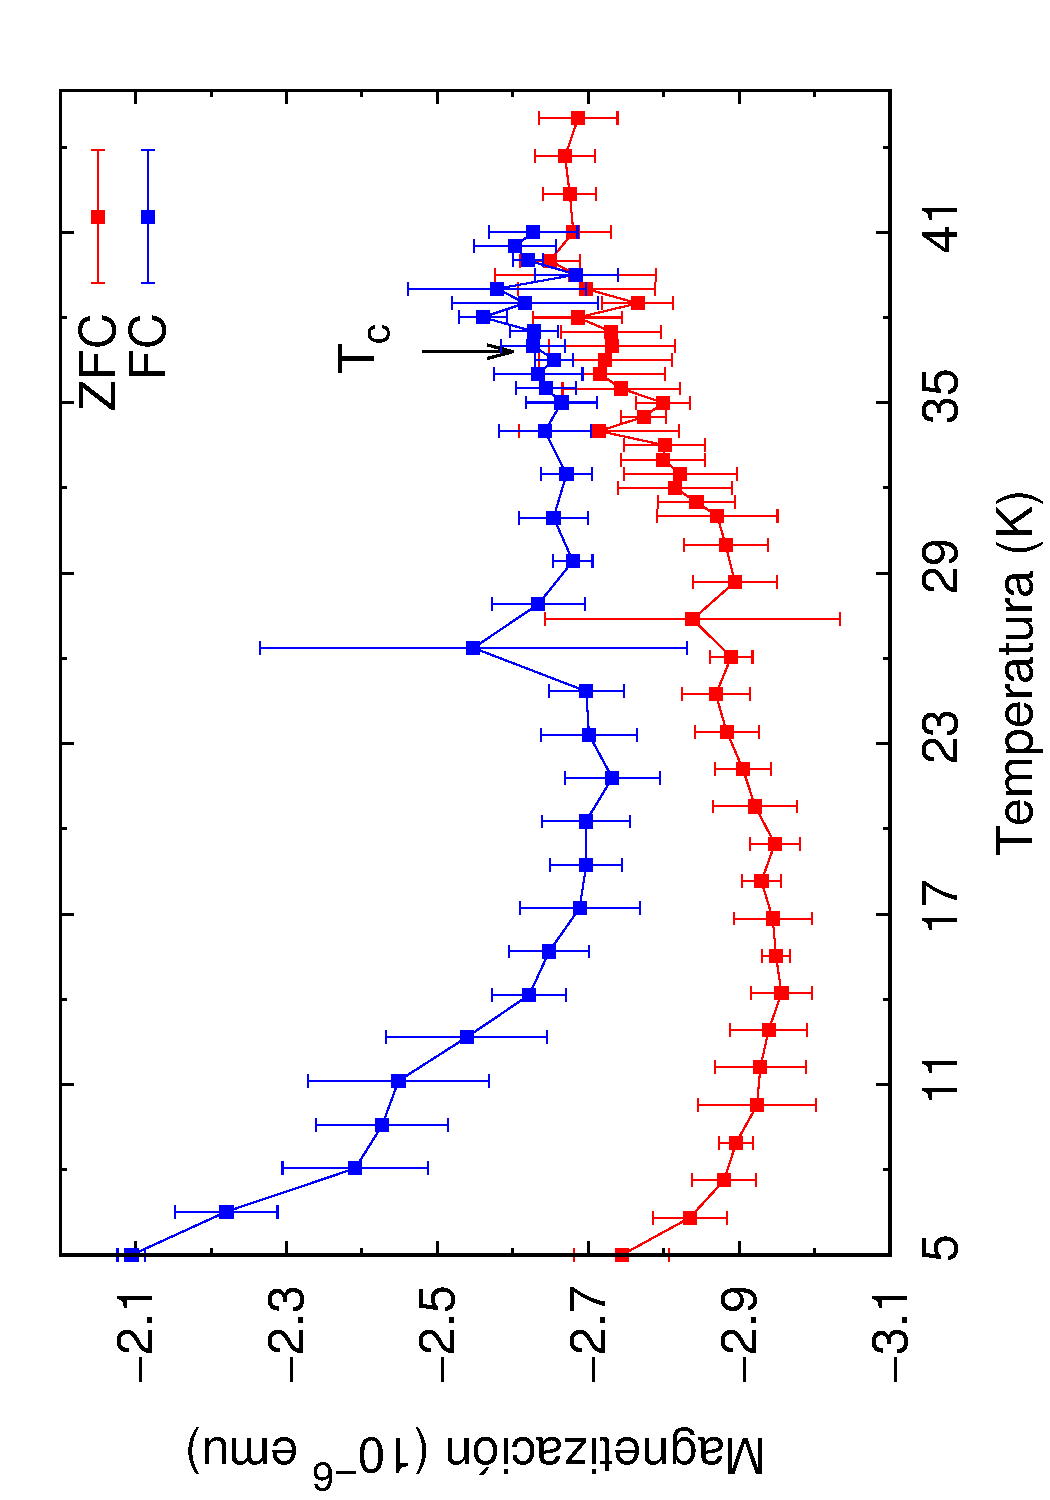
\includegraphics[width=0.5\columnwidth, angle=-90]{mgb2zaf}
  \end{center}
\caption[Magnetización en función de la temperatura para la muestra BBZ 1.]{Magnetización en función de la temperatura para la muestra BBZ 1. El sustrato es de zafiro. Al comparar con la Fig.\,\ref{fig:mgb2si}, puede apreciarse que en este caso la magnetización es negativa, y que la $T_c$ de este film también está entre 36\,K y 38\,K. Esto último es razonable, ya que ambas muestras fueron recocidas juntas.}
\label{fig:mgb2zaf}
\end{figure}

La figura\,\ref{fig:mgb2zaf} muestra la magnetización para un film de MgB$_2$ depositado sobre un sustrato de zafiro. Se aprecia una curva similar a la de la Fig.\,\ref{fig:mgb2si} aunque con magnetización negativa. Esto confirma la idea de que en el caso anterior, la magnetización positiva se deba al sustrato de Si.

También se midió el espesor de los films crecidos utilizando un perfilómetro mecánico de aguja. En la figura\,\ref{fig:histo2} se muestran las mediciones realizadas para la muestra BBZ 7. Para medir el espesor de los films se colocó pintura de plata en el sustrato antes de hacer la evaporación, y una vez realizada la misma, se removió la pintura, dejando expuesto un escalón que iba a permitir medir el espesor del film crecido. Luego se llevó la muestra cuyo espesor se deseaba determinar al perfilómetro mecánico, un equipo que consiste en una aguja que se puede mover en el plano de la muestra (plano xy), y que registra las variaciones en el eje perpendicular a ese plano (eje z) a partir de medir el desplazamiento vertical de la agua usando un sensor magnético. De las mediciones en el perfilómetro se obtuvieron perfiles como el que se ve en la Fig.\ref{fig:histo2}. Para cada muestra, se obtuvieron los perfiles de los escalones en diferentes lugares, y el espesor de los films se estimó de la siguiente forma: se ajustó una recta a cada nivel del escalón y luego se midió la distancia vertical entre dichas rectas en un punto del escalón. Se midió el espesor de los films antes del recocido y después de realizar el mismo. A partir de estas mediciones se estimó que la altura de los films de la 3ª evaporación tienen un espesor $d \, \approx \, 80 $\,nm, después de realizado el recocido. Mediciones análogas determinaron que la altura de los films de la 2ª evaporación es $d \, \approx \, 550 $\,nm, también después del recocido.

\begin{figure}[h!]
 \begin{center}
    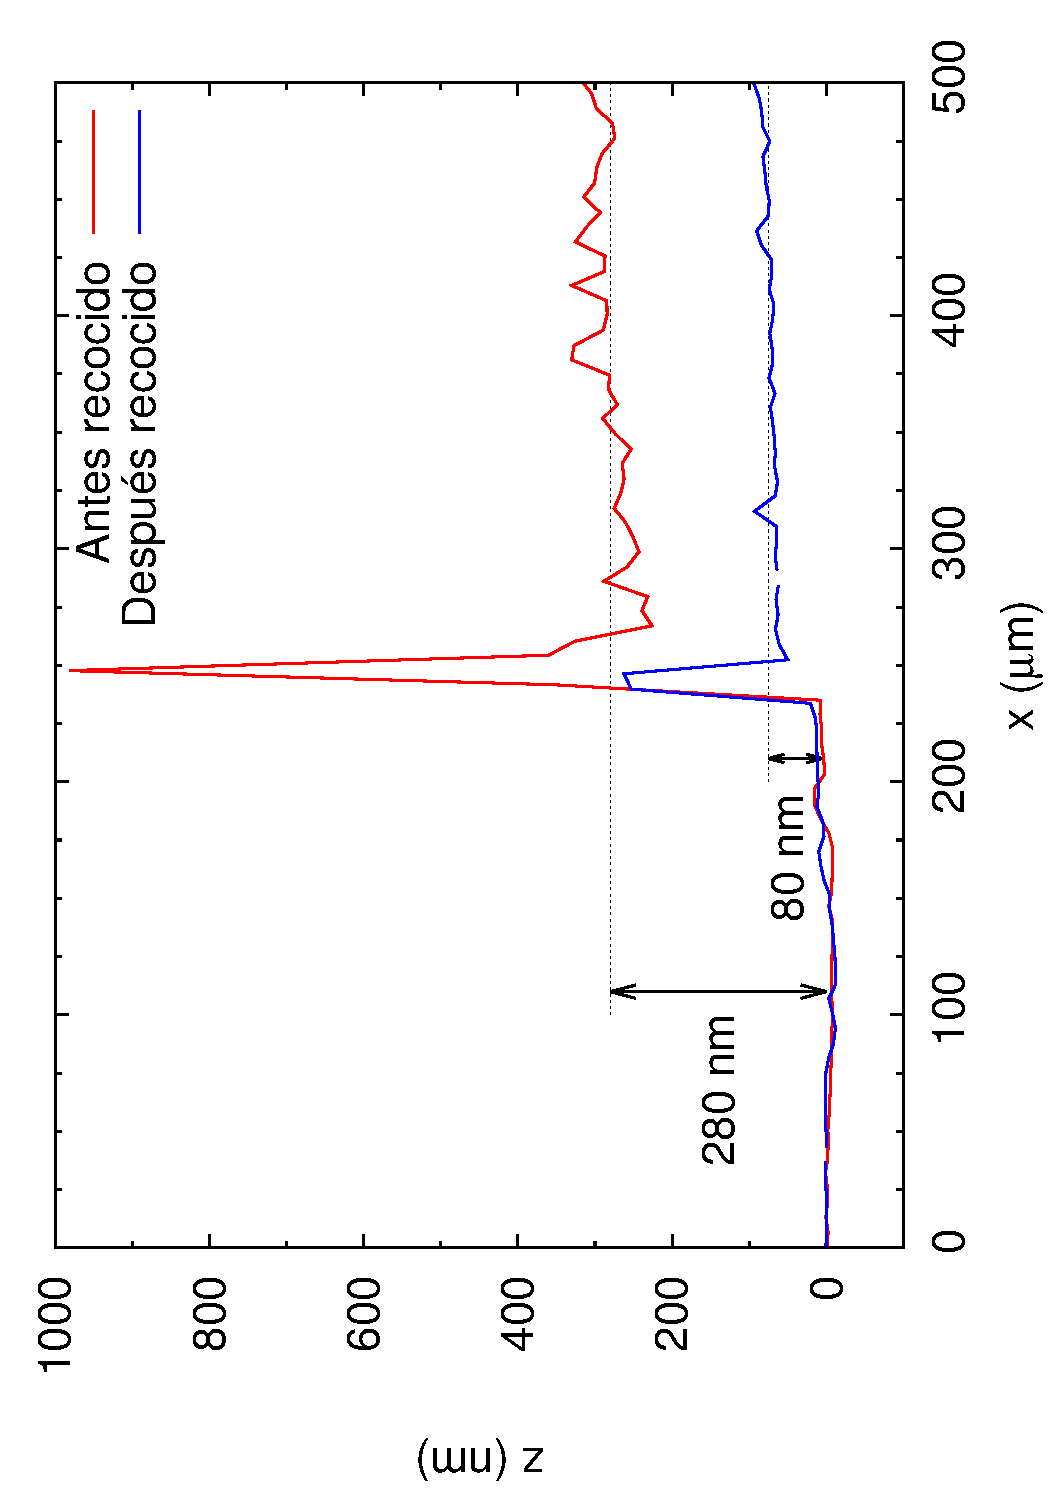
\includegraphics[width=0.5\columnwidth, angle=-90]{altura}
  \end{center}
\caption[Altura de los films de boro (antes del recocido) y de los MgB$_2$ (después del recocido).]{Altura de los films de boro (antes del recocido) y de los MgB$_2$ (después del recocido). Puede verse claramente que el espesor de los films disminuye notablemente después del recocido.}
\label{fig:histo2}
\end{figure}
%\newpage
En la Fig. \ref{fig:histo2} se compara la medición de la altura de la muestra BBZ 7 antes de realizar el recocido y después de realizar el mismo, lo que permite notar que los films se vuelven muchos más delgados después de ser recocidos. Se pensó que esto podía deberse a que parte del MgB$_2$ de la pastilla se depositaba en la parte descubierta del sustrato, lo que implicaría que la disminución del espesor del film es sólo aparente. En caso de ser cierto este supuesto, cabe entonces hacer la pregunta de si la irreversibilidad observada en las Figs \ref{fig:mgb2si} y \ref{fig:mgb2zaf} no es debida al MgB$_2$ que se depositó sobre los films. Para verificar esta hipótesis, se creció un film de boro con dos máscaras, una que se quitó antes del recocido y otra que se quitó después. Al hacer esto se pudo apreciar que es correcto pensar que algo del MgB$_2$ se deposita en el sustrato, pero lo que se deposita no es suficiente como para explicar la disminución observada en el espesor del film. Por otro lado se pensó que esta variación de alturas podía deberse a la diferencia de densidades del boro y el MgB$_2$, pero esta variación tampoco alcanza para explicar las variaciones medidas.

Investigando en la literatura que se encontró que es posible que debido a las altas temperaturas del recocido, parte del film difunda a través del sustrato \cite{Zhai1995, Naito2004, He2002}. En \cite{He2002} se muestra como el oxígeno presente en el zafiro reacciona con el Mg a temperaturas mayores a 600\,$^{\circ}$C, y esto resulta en una transición superconductora ancha. En el mismo trabajo también se muestra que el recocido con silicio da resultados parecidos.

\section{Análisis del método}\label{S:evapanalisis}
El método de evaporación y recocido realizado en este trabajo presenta como principal punto positivo el de que emplea un equipo relativamente sencillo de utilizar. Además, la $T_{c}$ de los films obtenidos no parece ser mucho peor que la de pastilla de MgB$_{2}$ utilizada para hacer los recocidos. Sin embargo, el método implementado en esta sección presenta algunos inconvenientes que deben ser tenidos en cuenta si se busca producir un dispositivo electrónico, siendo el primero la pobre adherencia que tienen los films con el sustrato, incluso después del recocido. Esto se debe a que los átomos de boro que se evaporan llegan al sustrato con una energía cinética del orden de la temperatura a la que se encuentra la naveta durante el crecimiento del film, es decir, algunas décimas de eV. Esto resulta en que el átomo que llega no posee la energía suficiente como para explorar el sustrato y acomodarse en la mejor región del mismo, y esto tiene como consecuencia que la adherencia entre el sustrato y el film no sea buena. El siguiente punto negativo es que para poder evaporar boro, se requiere poder calentar el mismo a temperaturas del orden de los miles de grados, y esto sólo se puede lograr utilizando una naveta de grafito, lo que introduce una fuente adicional del contaminación al proceso de crecimiento. Adicionalmente, el procedimiento experimental que hay que seguir para crecer los films no es del todo repetible de crecimiento a crecimiento. Se puede dar como ejemplo el recubrimiento de boro observado en las navetas de grafito (Fig. \ref{fig:nav}), que podía formarse o no, dependiendo de que tan rápido se caliente la naveta durante la evaporación. Por último, las altas temperaturas necesarias para el recocido llevan a que el MgB$_{2}$ que se pretende formar reaccione con el sustrato o difunda a través de él, y esto trae aparejado un ensanchamiento de la transición superconductora. Entonces, si se busca desarrollar un dispositivo electrónico es preciso evitar el paso de recocido o bajar la temperatura a la que ocurre el mismo, así como es necesario un método de depósito que sea más fácilmente reproducible y que permita lograr un film con mejor adherencia. En la sección siguiente se explora la posibilidad de crecer films de MgB$_{2}$ directamente por sputtering, un método que permite lograr films que tienen una excelente adherencia con el sustrato, gracias que las partículas llegan al sustrato con energías del orden los eV. 
